{\color{gray}\hrule}
\begin{center}
\section{Theory}
\bigskip
\end{center}
{\color{gray}\hrule}

\begin{multicols}{2}
\subsection{Introduction to general rotations}
\label{sec:theory:introduction}

Similarly to translations, there are equivalent equations for rotations:
\begin{itemize}
\item \emph{Velocity Addition} / \emph{Angular Velocity Addition}: $$\boldsymbol\omega_{1,3} = \boldsymbol\omega_{1,2} + \boldsymbol\omega_{2,3}$$
\item \emph{Momentum} / \emph{Angular Momentum}: $$\mathbf{L} = \int \mathbf{r} \times (\boldsymbol\omega \times \mathbf{r}) dm = \mathbf{I} \boldsymbol\omega$$
\item \emph{Mass} / \emph{Inertia Moment}: $$\mathbf{I} = \begin{pmatrix} I_{xx} & I_{xy} & I_{xz} \\ I_{yx} & I_{yy} & I_{yz} \\ I_{zx} & I_{zy} & I_{zz} \end{pmatrix}$$
\item \emph{Kinetic Energy}: $$T = \frac{1}{2} \boldsymbol\omega \cdot \mathbf{L} $$
\item \emph{Force} / \emph{Torque}: $$\boldsymbol\tau = \mathbf{r} \times \mathbf{F} = \frac{d\mathbf{L}}{dt} = \mathbf{I}\frac{d\boldsymbol\omega}{dt}$$
\end{itemize}

Thus, one must calculate each component in the inertia tensor ($\mathbf{I}$) depending on the coordinate system\footnote{The origin of the coordinate system is arbitrary.} to compute the net torque ($\boldsymbol{\tau}$). However, there always exists a set of principal axes\footnote{For every origin, there exists a set of principal axes} (see Section 9.3 \cite{morin}) for which all the off-diagonal components of $\mathbf{I}$ tensor are zero. Thus, $I$ reduces to $diag \begin{pmatrix} I_{xx} & I_{yy} & I_{zz} \end{pmatrix}$. There are two important consequences:
\begin{itemize}
\item $\mathbf{L}$ is aligned with the net $\boldsymbol\omega$, because the principal inertia tensor only scales $\boldsymbol\omega$.\footnote{In general, angular momentum is not collinear with angular velocity.}
\item A rigid body \emph{likes} rotating around principal axes (that is, $\boldsymbol\tau = \mathbf{0}$).
\end{itemize}

If one calculated quantities associated with rotations around CM, equations shown below relate those quantities with respect to other origins as discussed in pp. 380-383 \cite{morin}.
\begin{itemize}
\item \emph{Angular Momentum}: $\mathbf{L} = M(\mathbf{R} \times \mathbf{V}) + \mathbf{L}_{CM}$
\item \emph{Kinetic Energy}: $T = \frac{1}{2}MV^2 + \frac{1}{2}\boldsymbol\omega \cdot \mathbf{L}_{CM}$
\item \emph{Parallel-axis theorem}: $\mathbf{L} = \left( \mathbf{I}_{R} + \mathbf{I}_{CM} \right) \boldsymbol\omega$
\end{itemize}

Gyroscope consists of the homogeneous heavy cylindrical rotor of radius $R_{d}$ and mass $M_{d}$. For this lab, relevant inertia moment is calculated with respect to its symmetry axis. In cylindrical coordinates, the inertia moment is:
\begin{equation*}
  I = \int_{m}r^{2}dm = \rho\int_{0}^{H} \int_{0}^{2\pi}\int_{0}^{R_d}r^{2} rdrd\theta dz 
\end{equation*}
where
\begin{equation*}
  \rho = \frac{M_{d}}{V} = \frac{M_{d}}{\pi R_{d}^{2} H}
\end{equation*}
\begin{equation} \label{eq:theory:id}
  I = \frac{M_{d}}{\pi R_{d}^{2} H} \times H \times 2\pi \times \frac{R_{d}^{4}}{4} \Rightarrow I_{d} = \frac{1}{2} M_{d} R_{d}^{2}
\end{equation}

\subsection{Precession}
\label{sec:theory:precession}

In precession, a heavy symmetrical top (see figure \ref{fig:theory:top}) keeps a constant angle $\theta$ with the vertical $\hat{z}$ by rotating around this axis with angular velocity $\boldsymbol\Omega = \Omega \hat{z}$, and spinning around its symmetry axis $\hat{x_{3}}$ with angular velocity $\boldsymbol\omega_{3} = \omega_{3} \hat{x_{3}}$. Since a heavy symmetric top is symmetrical around $\hat{x_{3}}$, this axis is its principal axis. All other axes (e.g., $\hat{x_{2}}$ and $\hat{x_{1}}$) orthogonal to $\hat{x_{3}}$ are also principal if the origin lies on the $\hat{x_{3}}$ axis (see Section 9.6 and Section 9.3 Theorem 9.5-9.6 \cite{morin} for more details).

\begin{figure}[H]
  \centering
  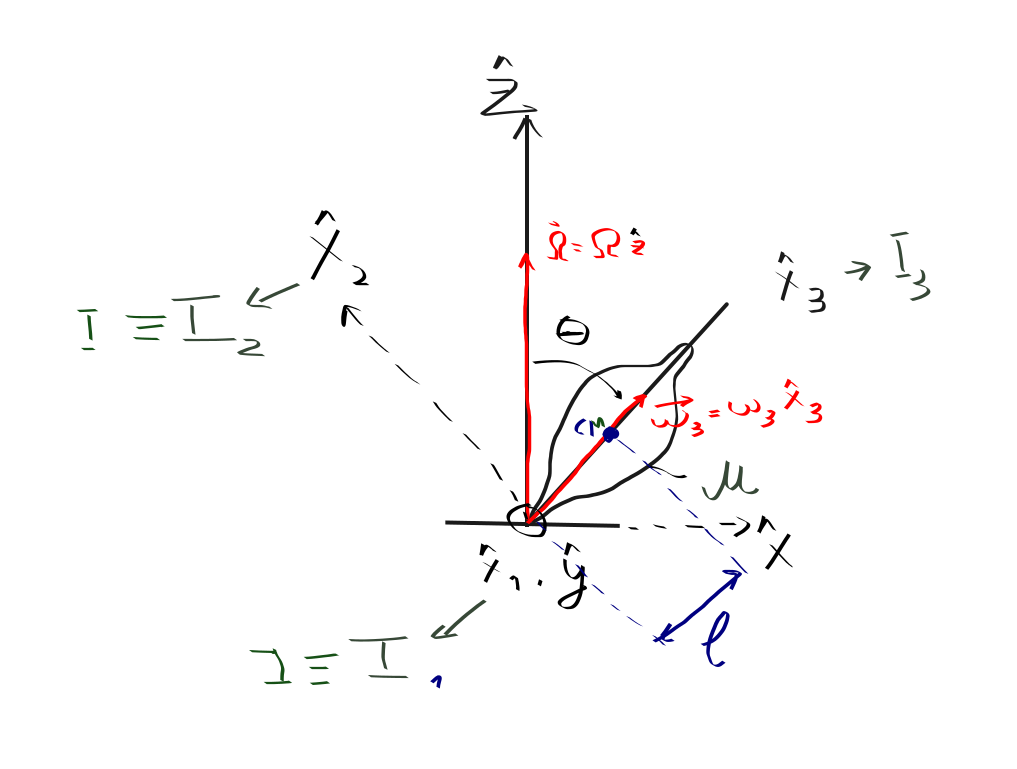
\includegraphics[width=\columnwidth]{gyroscope/images/top}
  \caption{A heavy symmetrical top}
  \label{fig:theory:top}
\end{figure}

For the system in figure \ref{fig:theory:top}, the precession frequency $\Omega$ and the spinning $\omega$ are related by (see Section 9.7 \cite{morin} for derivation):
\begin{equation*}
  \Omega_{\pm} = \frac{I_{3}\omega_3}{2I\cos(\theta)} \left( 1 \pm \sqrt{1 - \frac{4MIgl\cos(\theta)}{I_{3}^{2} \omega_{3}^{2}}}  \right)
\end{equation*}
where
\begin{itemize}
\item $I$: inertia moment of the heavy symmetric top around $\hat{x_{2}}$ or $\hat{x_{1}}$ ($I_{1} = I_{2} = I$)
\item $I_{3}$: inertia moment of the heavy symmetric top around $\hat{x_{3}}$
\item $M$: mass of the top
\item $l$: distance from the pivot to CM of the top
\end{itemize}

However, in this lab report an approximate relation for large $\omega_{3}$ is used.
\begin{equation}
  \label{eq:theory:precession_frequency}
  \Omega \approx \frac{Mgl}{I_{3}\omega_{3}}
\end{equation}

Then, precession period is
\begin{equation}
  \label{eq:theory:precession_period}
  T_{p} = \frac{2\pi}{\Omega} = \frac{2\pi I_{3} \omega_3}{Mgl} = \frac{4\pi^{2} I_{3}}{MglT_{3}}
\end{equation}
where $\omega_{3} = \frac{2\pi}{T_{3}}$.

\subsection{Nutation}
\label{sec:theory:nutation}

Nutation is a phenomenon where $\theta$ is not constant but it fluctuates around some value with angular velocity $\omega_{n}$. Since nutation is often coupled with precession, the top precesses in an ellipse around $\hat{z}$ axis. Nutation angular velocity $\omega_{n}$ and $\theta$ are given by:
\begin{equation}
  \label{eq:theory:nutation_frequency}
  \omega_{n} = \frac{I_{3}\omega_3}{I}
\end{equation}
\begin{equation*}
  \theta(t) = B + (\frac{A}{\omega_n}\sin \theta_{0})\cos(\omega_{n}t + \gamma), \left\{ A, B, \theta_{0}, \gamma \right\} \subset \mathbb{R}
\end{equation*}

\end{multicols}
